\section{Kommunikation}

\subsection{Client <-> Server} 
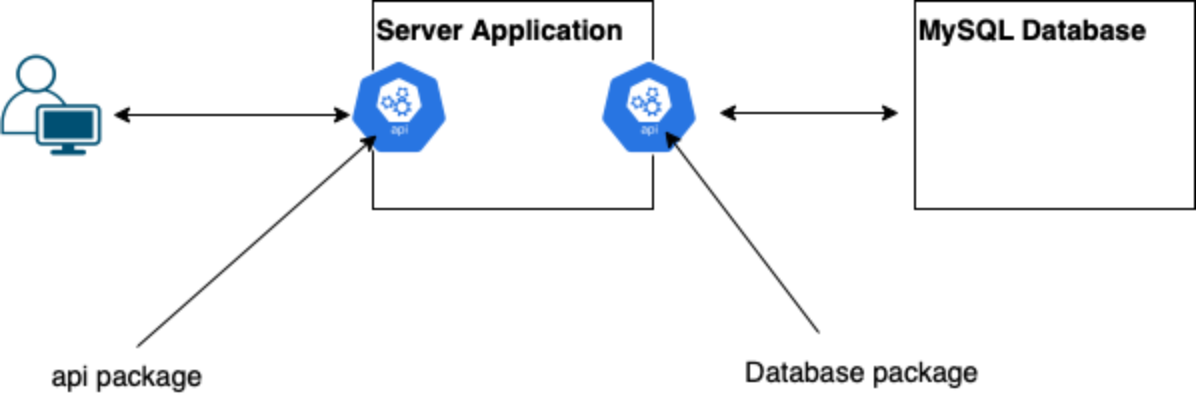
\includegraphics[width=1\textwidth]{res/Kommunikation.png}
Die Kommunikation zwischen Client und Server erfolgt über das \nameref{API}, bei der die Klasse FrontendAPI 
als RESTful API über JSON mit dem Client kommuniziert und das Database Package die Kommunikation 
zwischen der Datenbank und der Server Application regelt.

%Frontend API
Mithilfe von Flask läuft auf dem Hostserver eine RESTful API, die 

%Lukas zum Database package

\subsection{Server <-> Airflow API}

\newpage